\chapter{RL \& RL Training }
%\label{chapter:title}
\section{Overview of RL Algorithms}\label{section:RL aglorithms overview}
Various RL algorithms exist to solve the MDP problem as discussed above (\autoref{rl_fundamentals}). There are two main categories which exist in RL, model-based and model-free. Where model free reinforcement learning solely learns from the interactions between the agent and the environment, without any knowledge of the underlying dynamics. Both have been successfully applied in the greenhouse control problem with model-based RL being used in \cite{zhangRobustModelbasedReinforcement2021,} and model-free in \cite{jansenOptimalControlLettuce2023,ajagekarDeepReinforcementLearning2022,vandenbemdRobustDeepReinforcement,hemmingRemoteControlGreenhouse2019}. Both offer their respective advantages and disadvantages. Most commonly, since model-based reinforcement learning encodes the dynamics of the environment, it offers efficient sampling and faster learning since it allows the agent to plan its action ahead of time, whereas model-free has shown to have better asymptotic performance in complex environments. An interesting model-based algorithm as used in Alpha-Zero \cite{silverGeneralReinforcementLearning2018}, 
utilizes a known model, where the policy is planned over the known model and horizon but uses learning for the global solution.\cite{jonkerModelbasedReinforcementLearning}. Alpha-Zero was considered the best chess engine upon its release and continues to be recognized as one of the top contenders \cite{silverGeneralReinforcementLearning2018}. However the ground-truth model of the environment is usually not available, and therefore only the simplified dynamics is used in model-based RL. However, model-free is able to learn the model only from experience. 

Additionally, model-free algorithms may be classified into two further categories: Policy Gradient methods (Policy Optimization) and Q-learning. Actor-Critic algorithms are an amalgamation of the two. \autoref{fig:rl_taxonomy} displays an overview of the non-exhaustive taxonomy of RL algorithms. These RL algorithms (\autoref{fig:rl_taxonomy}) are used to  learn a various aspects (or a combination) of the MDP. These aspects encompass policies (both stochastic and deterministic), Q-functions, value functions, and/or environment models.

%insert taxonomy of algoirthms and talk about them.
\begin{figure}[h]
	\centering
	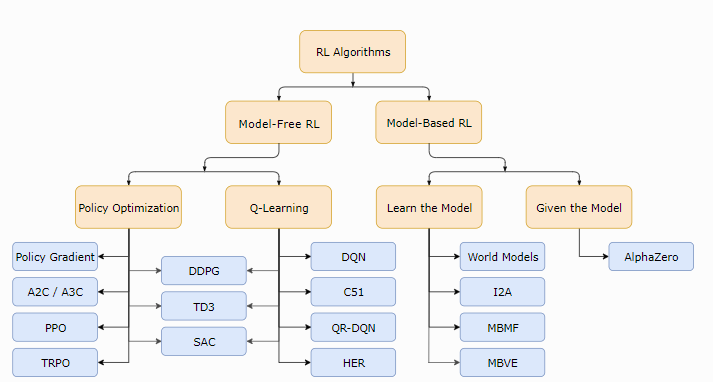
\includegraphics{figures/rl_taxonomy.png}
	\caption{Taxonomy of algorithms in modern RL}
	\label{fig:rl_taxonomy}
\end{figure}

This thesis will explore a model-based method of RL.It is imperative to understand both Q-learning and Policy Optimization (and actor-critic methods),  although the developed algorithm may be classified as model-based, model-free RL techniques are used to gain an estimation of the value function. 


\section{Selection of RL Algorithm} \label{section:selection of RL algorithm}
In order to select an RL algorithm, it must first be determined what is needed from the respective algorithm. Since the objective of the thesis is to combine RL with MPC with RL as the initial approximate solution to the MPC problem, a value function is required. This value function can either be a Q-function or a State value function. Moreover, the approximated value function needs to accommodate continuous states and actions. \autoref{greenhouse_model} outlines the environment, and due to the numerous state variables and actions available, discretizing either the action or state space (or both) would lead to a rapid increase in the dimensionality of the problem (curse of dimensionality). Hence a suitable approach would be the use of actor-critic or policy optimization methods. 


All model-free algorithms presented in \autoref{fig:rl_taxonomy}, except for (Vanilla) Policy Gradient, utilizes an approximated value function. Although A2C/A3C, PPO and TRPO are classified as policy optimization approaches, they are commonly used with critic-networks to reduce variance and increase learning speed, as opposed to using monte-carlo sampling \cite{suttonReinforcementLearningIntroduction2014}.

In recent developments, q-learning algorithms such as DQN (developed in 2013 \cite{mnihAsynchronousMethodsDeep2016}), originally designed for discrete actions \cite{suttonReinforcementLearningIntroduction2014}, have been extended with Deterministic Policy Gradient approaches \cite{silverDeterministicPolicyGradient} to be capable of continuous action spaces. The resulting actor-critic algorithm, known as Deep Deterministic Policy Gradient (DDPG) \cite{lillicrapContinuousControlDeep2019}, is an off-policy algorithm capable of both continuous state and action spaces  and was developed in 2016. 

Furthermore, a policy optimization method, TRPO, was released in 2015 \cite{schulmanTrustRegionPolicy2017} and improved upon the stability and learning speed of vanilla policy gradients by limiting the size of the policy update, although it is a challenging algorithm to implement. The Kullback Leibler (KL) Divergence is applied to ensure that the updated policy does not differ significantly from the previous policy.

In 2016, (Asynchronous) Advantage Actor-Critic A2C/A3C was published \cite{mnihAsynchronousMethodsDeep2016}, whereby A3C is an asynchronous version of A2C. A2C/A3C is on-policy policy optimization algorithm, that uses a value function to optimize the policy gradients. A3C significantly reduces the time of learning by using multiple agents to gather experience to update the shared policy network. The gathered experience is more diverse which stabilizes training as compared to A2C. However, it was found empirically that A2C produces comparable performance to A3C while being more efficient \cite{yoonUnderstandingActorCritic2019}.


Proximal Policy Optimization (PPO) was released to further improve on TRPO in 2017 \cite{schulmanProximalPolicyOptimization2017}. Instead of using KL divergence to restrict the size of the policy update, first order methods are used to limit the update policy, allowing for easier implementation,faster learning and similar performance.

Finally, in 2018, two algorithms were released. Twin Delayed Deep Deterministic Policy Gradient (TD3) was introduced \cite{fujimotoAddressingFunctionApproximation2018} and expands on the DDPG algorithm. TD3 uses additional Q-functions, delayed updates and policy smoothing to improve the performance and the stability of the DDPG algorithm. Moreover, Soft Actor-Critic (SAC) also extends the framework established by DDPG, but uses entropy regularization for agent exploration and removes the need for policy smoothing. Additional differences are in the way the agents actions are selected during learning, where TD3 uses the target policy, SAC uses the current policy. However, both algorithms are considered state-of-the-art algorithms and have similar performance, with SAC having a slightly faster convergence rate due to its entropy regularization. 

Algorithms such as A2C/A3C \cite{mnihAsynchronousMethodsDeep2016}, PPO \cite{schulmanProximalPolicyOptimization2017} and TRPO \cite{schulmanTrustRegionPolicy2017}, are on-policy methods, albeit state-of-the-art algorithms, have low sample efficiency and high computational cost. The greenhouse is a complex environment and the anticipated  learning process for policies in such a complex setting is expected to be long, therefore opting for an off-policy method is deemed desirable. Both Twin-Delayed Deep Deterministic Policy Gradient (TD3) \cite{fujimotoAddressingFunctionApproximation2018} and Soft Actor-Critic (SAC) \cite{haarnojaSoftActorCriticOffPolicy2018} are extensions of DDPG that result in a more stable Q-function and thus it was decided to use SAC.

\section{Agent Training}

\section{Value Function Training}